\documentclass[1p]{elsarticle_modified}
%\bibliographystyle{elsarticle-num}

%\usepackage[colorlinks]{hyperref}
%\usepackage{abbrmath_seonhwa} %\Abb, \Ascr, \Acal ,\Abf, \Afrak
\usepackage{amsfonts}
\usepackage{amssymb}
\usepackage{amsmath}
\usepackage{amsthm}
\usepackage{scalefnt}
\usepackage{amsbsy}
\usepackage{kotex}
\usepackage{caption}
\usepackage{subfig}
\usepackage{color}
\usepackage{graphicx}
\usepackage{xcolor} %% white, black, red, green, blue, cyan, magenta, yellow
\usepackage{float}
\usepackage{setspace}
\usepackage{hyperref}

\usepackage{tikz}
\usetikzlibrary{arrows}

\usepackage{multirow}
\usepackage{array} % fixed length table
\usepackage{hhline}

%%%%%%%%%%%%%%%%%%%%%
\makeatletter
\renewcommand*\env@matrix[1][\arraystretch]{%
	\edef\arraystretch{#1}%
	\hskip -\arraycolsep
	\let\@ifnextchar\new@ifnextchar
	\array{*\c@MaxMatrixCols c}}
\makeatother %https://tex.stackexchange.com/questions/14071/how-can-i-increase-the-line-spacing-in-a-matrix
%%%%%%%%%%%%%%%

\usepackage[normalem]{ulem}

\newcommand{\msout}[1]{\ifmmode\text{\sout{\ensuremath{#1}}}\else\sout{#1}\fi}
%SOURCE: \msout is \stkout macro in https://tex.stackexchange.com/questions/20609/strikeout-in-math-mode

\newcommand{\cancel}[1]{
	\ifmmode
	{\color{red}\msout{#1}}
	\else
	{\color{red}\sout{#1}}
	\fi
}

\newcommand{\add}[1]{
	{\color{blue}\uwave{#1}}
}

\newcommand{\replace}[2]{
	\ifmmode
	{\color{red}\msout{#1}}{\color{blue}\uwave{#2}}
	\else
	{\color{red}\sout{#1}}{\color{blue}\uwave{#2}}
	\fi
}

\newcommand{\Sol}{\mathcal{S}} %segment
\newcommand{\D}{D} %diagram
\newcommand{\A}{\mathcal{A}} %arc


%%%%%%%%%%%%%%%%%%%%%%%%%%%%%5 test

\def\sl{\operatorname{\textup{SL}}(2,\Cbb)}
\def\psl{\operatorname{\textup{PSL}}(2,\Cbb)}
\def\quan{\mkern 1mu \triangleright \mkern 1mu}

\theoremstyle{definition}
\newtheorem{thm}{Theorem}[section]
\newtheorem{prop}[thm]{Proposition}
\newtheorem{lem}[thm]{Lemma}
\newtheorem{ques}[thm]{Question}
\newtheorem{cor}[thm]{Corollary}
\newtheorem{defn}[thm]{Definition}
\newtheorem{exam}[thm]{Example}
\newtheorem{rmk}[thm]{Remark}
\newtheorem{alg}[thm]{Algorithm}

\newcommand{\I}{\sqrt{-1}}
\begin{document}

%\begin{frontmatter}
%
%\title{Boundary parabolic representations of knots up to 8 crossings}
%
%%% Group authors per affiliation:
%\author{Yunhi Cho} 
%\address{Department of Mathematics, University of Seoul, Seoul, Korea}
%\ead{yhcho@uos.ac.kr}
%
%
%\author{Seonhwa Kim} %\fnref{s_kim}}
%\address{Center for Geometry and Physics, Institute for Basic Science, Pohang, 37673, Korea}
%\ead{ryeona17@ibs.re.kr}
%
%\author{Hyuk Kim}
%\address{Department of Mathematical Sciences, Seoul National University, Seoul 08826, Korea}
%\ead{hyukkim@snu.ac.kr}
%
%\author{Seokbeom Yoon}
%\address{Department of Mathematical Sciences, Seoul National University, Seoul, 08826,  Korea}
%\ead{sbyoon15@snu.ac.kr}
%
%\begin{abstract}
%We find all boundary parabolic representation of knots up to 8 crossings.
%
%\end{abstract}
%\begin{keyword}
%    \MSC[2010] 57M25 
%\end{keyword}
%
%\end{frontmatter}

%\linenumbers
%\tableofcontents
%
\newcommand\colored[1]{\textcolor{white}{\rule[-0.35ex]{0.8em}{1.4ex}}\kern-0.8em\color{red} #1}%
%\newcommand\colored[1]{\textcolor{white}{ #1}\kern-2.17ex	\textcolor{white}{ #1}\kern-1.81ex	\textcolor{white}{ #1}\kern-2.15ex\color{red}#1	}

{\Large $\underline{12n_{0477}~(K12n_{0477})}$}

\setlength{\tabcolsep}{10pt}
\renewcommand{\arraystretch}{1.6}
\vspace{1cm}\begin{tabular}{m{100pt}>{\centering\arraybackslash}m{274pt}}
\multirow{5}{120pt}{
	\centering
	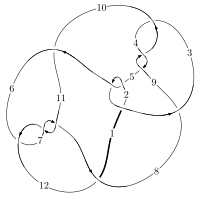
\includegraphics[width=112pt]{../../../GIT/diagram.site/Diagrams/png/2566_12n_0477.png}\\
\ \ \ A knot diagram\footnotemark}&
\allowdisplaybreaks
\textbf{Linearized knot diagam} \\
\cline{2-2}
 &
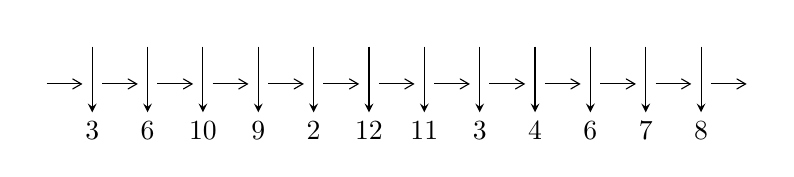
\begin{tikzpicture}[x=20pt, y=17pt]
	% nodes
	\node (C0) at (0, 0) {};
	\node (C1) at (1, 0) {};
	\node (C1U) at (1, +1) {};
	\node (C1D) at (1, -1) {3};

	\node (C2) at (2, 0) {};
	\node (C2U) at (2, +1) {};
	\node (C2D) at (2, -1) {6};

	\node (C3) at (3, 0) {};
	\node (C3U) at (3, +1) {};
	\node (C3D) at (3, -1) {10};

	\node (C4) at (4, 0) {};
	\node (C4U) at (4, +1) {};
	\node (C4D) at (4, -1) {9};

	\node (C5) at (5, 0) {};
	\node (C5U) at (5, +1) {};
	\node (C5D) at (5, -1) {2};

	\node (C6) at (6, 0) {};
	\node (C6U) at (6, +1) {};
	\node (C6D) at (6, -1) {12};

	\node (C7) at (7, 0) {};
	\node (C7U) at (7, +1) {};
	\node (C7D) at (7, -1) {11};

	\node (C8) at (8, 0) {};
	\node (C8U) at (8, +1) {};
	\node (C8D) at (8, -1) {3};

	\node (C9) at (9, 0) {};
	\node (C9U) at (9, +1) {};
	\node (C9D) at (9, -1) {4};

	\node (C10) at (10, 0) {};
	\node (C10U) at (10, +1) {};
	\node (C10D) at (10, -1) {6};

	\node (C11) at (11, 0) {};
	\node (C11U) at (11, +1) {};
	\node (C11D) at (11, -1) {7};

	\node (C12) at (12, 0) {};
	\node (C12U) at (12, +1) {};
	\node (C12D) at (12, -1) {8};
	\node (C13) at (13, 0) {};

	% arrows
	\draw[->,>={angle 60}]
	(C0) edge (C1) (C1) edge (C2) (C2) edge (C3) (C3) edge (C4) (C4) edge (C5) (C5) edge (C6) (C6) edge (C7) (C7) edge (C8) (C8) edge (C9) (C9) edge (C10) (C10) edge (C11) (C11) edge (C12) (C12) edge (C13) ;	\draw[->,>=stealth]
	(C1U) edge (C1D) (C2U) edge (C2D) (C3U) edge (C3D) (C4U) edge (C4D) (C5U) edge (C5D) (C6U) edge (C6D) (C7U) edge (C7D) (C8U) edge (C8D) (C9U) edge (C9D) (C10U) edge (C10D) (C11U) edge (C11D) (C12U) edge (C12D) ;
	\end{tikzpicture} \\
\hhline{~~} \\& 
\textbf{Solving Sequence} \\ \cline{2-2} 
 &
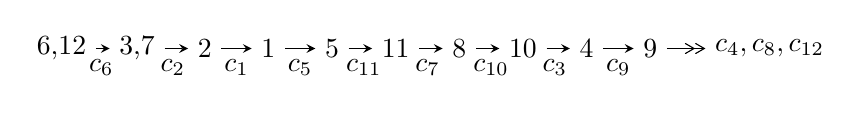
\begin{tikzpicture}[x=23pt, y=7pt]
	% node
	\node (A0) at (-1/8, 0) {6,12};
	\node (A1) at (17/16, 0) {3,7};
	\node (A2) at (17/8, 0) {2};
	\node (A3) at (25/8, 0) {1};
	\node (A4) at (33/8, 0) {5};
	\node (A5) at (41/8, 0) {11};
	\node (A6) at (49/8, 0) {8};
	\node (A7) at (57/8, 0) {10};
	\node (A8) at (65/8, 0) {4};
	\node (A9) at (73/8, 0) {9};
	\node (C1) at (1/2, -1) {$c_{6}$};
	\node (C2) at (13/8, -1) {$c_{2}$};
	\node (C3) at (21/8, -1) {$c_{1}$};
	\node (C4) at (29/8, -1) {$c_{5}$};
	\node (C5) at (37/8, -1) {$c_{11}$};
	\node (C6) at (45/8, -1) {$c_{7}$};
	\node (C7) at (53/8, -1) {$c_{10}$};
	\node (C8) at (61/8, -1) {$c_{3}$};
	\node (C9) at (69/8, -1) {$c_{9}$};
	\node (A10) at (11, 0) {$c_{4},c_{8},c_{12}$};

	% edge
	\draw[->,>=stealth]	
	(A0) edge (A1) (A1) edge (A2) (A2) edge (A3) (A3) edge (A4) (A4) edge (A5) (A5) edge (A6) (A6) edge (A7) (A7) edge (A8) (A8) edge (A9) ;
	\draw[->>,>={angle 60}]	
	(A9) edge (A10);
\end{tikzpicture} \\ 

\end{tabular} \\

\footnotetext{
The image of knot diagram is generated by the software ``\textbf{Draw programme}" developed by Andrew Bartholomew(\url{http://www.layer8.co.uk/maths/draw/index.htm\#Running-draw}), where we modified some parts for our purpose(\url{https://github.com/CATsTAILs/LinksPainter}).
}\phantom \\ \newline 
\centering \textbf{Ideals for irreducible components\footnotemark of $X_{\text{par}}$} 
 
\begin{align*}
I^u_{1}&=\langle 
-2225017 u^{29}+4505754 u^{28}+\cdots+4816957 b-1955093,\\
\phantom{I^u_{1}}&\phantom{= \langle  }-2648086 u^{29}-9433003 u^{28}+\cdots+28901742 a+37209631,\;u^{30}-2 u^{29}+\cdots+5 u-3\rangle \\
I^u_{2}&=\langle 
b-1,\;-2 u^2 a+a^2-2 a u+4 u^2-4 a+3 u+7,\;u^3+u^2+2 u+1\rangle \\
I^u_{3}&=\langle 
b+1,\;u^2+a- u+2,\;u^3- u^2+2 u-1\rangle \\
\\
\end{align*}
\raggedright * 3 irreducible components of $\dim_{\mathbb{C}}=0$, with total 39 representations.\\
\footnotetext{All coefficients of polynomials are rational numbers. But the coefficients are sometimes approximated in decimal forms when there is not enough margin.}
\newpage
\renewcommand{\arraystretch}{1}
\centering \section*{I. $I^u_{1}= \langle -2.23\times10^{6} u^{29}+4.51\times10^{6} u^{28}+\cdots+4.82\times10^{6} b-1.96\times10^{6},\;-2.65\times10^{6} u^{29}-9.43\times10^{6} u^{28}+\cdots+2.89\times10^{7} a+3.72\times10^{7},\;u^{30}-2 u^{29}+\cdots+5 u-3 \rangle$}
\flushleft \textbf{(i) Arc colorings}\\
\begin{tabular}{m{7pt} m{180pt} m{7pt} m{180pt} }
\flushright $a_{6}=$&$\begin{pmatrix}1\\0\end{pmatrix}$ \\
\flushright $a_{12}=$&$\begin{pmatrix}0\\u\end{pmatrix}$ \\
\flushright $a_{3}=$&$\begin{pmatrix}0.0916238 u^{29}+0.326382 u^{28}+\cdots-0.0897393 u-1.28745\\0.461913 u^{29}-0.935394 u^{28}+\cdots+0.0723297 u+0.405877\end{pmatrix}$ \\
\flushright $a_{7}=$&$\begin{pmatrix}1\\u^2\end{pmatrix}$ \\
\flushright $a_{2}=$&$\begin{pmatrix}0.553537 u^{29}-0.609012 u^{28}+\cdots-0.0174096 u-0.881576\\0.461913 u^{29}-0.935394 u^{28}+\cdots+0.0723297 u+0.405877\end{pmatrix}$ \\
\flushright $a_{1}=$&$\begin{pmatrix}- u^5-2 u^3- u\\- u^7-3 u^5-2 u^3+u\end{pmatrix}$ \\
\flushright $a_{5}=$&$\begin{pmatrix}0.847386 u^{29}-1.24384 u^{28}+\cdots-1.07511 u+1.57925\\0.551237 u^{29}-1.21563 u^{28}+\cdots-1.81025 u+0.917412\end{pmatrix}$ \\
\flushright $a_{11}=$&$\begin{pmatrix}u\\u^3+u\end{pmatrix}$ \\
\flushright $a_{8}=$&$\begin{pmatrix}u^2+1\\u^4+2 u^2\end{pmatrix}$ \\
\flushright $a_{10}=$&$\begin{pmatrix}u^3+2 u\\u^3+u\end{pmatrix}$ \\
\flushright $a_{4}=$&$\begin{pmatrix}-0.0573861 u^{29}+0.274952 u^{28}+\cdots+0.731599 u-2.38174\\0.0837160 u^{29}-0.147522 u^{28}+\cdots+1.77910 u-0.712657\end{pmatrix}$ \\
\flushright $a_{9}=$&$\begin{pmatrix}0.348620 u^{29}-1.11181 u^{28}+\cdots-3.98425 u+2.17901\\0.0392597 u^{29}-0.428436 u^{28}+\cdots-1.44021 u+0.962791\end{pmatrix}$\\&\end{tabular}
\flushleft \textbf{(ii) Obstruction class $= -1$}\\~\\
\flushleft \textbf{(iii) Cusp Shapes $= -\frac{4602334}{4816957} u^{29}+\frac{5525451}{4816957} u^{28}+\cdots-\frac{80618534}{4816957} u-\frac{73845258}{4816957}$}\\~\\
\newpage\renewcommand{\arraystretch}{1}
\flushleft \textbf{(iv) u-Polynomials at the component}\newline \\
\begin{tabular}{m{50pt}|m{274pt}}
Crossings & \hspace{64pt}u-Polynomials at each crossing \\
\hline $$\begin{aligned}c_{1}\end{aligned}$$&$\begin{aligned}
&u^{30}+42 u^{29}+\cdots+4660 u+289
\end{aligned}$\\
\hline $$\begin{aligned}c_{2},c_{5}\end{aligned}$$&$\begin{aligned}
&u^{30}+4 u^{29}+\cdots+28 u-17
\end{aligned}$\\
\hline $$\begin{aligned}c_{3},c_{4},c_{9}\end{aligned}$$&$\begin{aligned}
&u^{30}- u^{29}+\cdots+16 u+8
\end{aligned}$\\
\hline $$\begin{aligned}c_{6},c_{7},c_{11}\end{aligned}$$&$\begin{aligned}
&u^{30}+2 u^{29}+\cdots-5 u-3
\end{aligned}$\\
\hline $$\begin{aligned}c_{8}\end{aligned}$$&$\begin{aligned}
&u^{30}+u^{29}+\cdots-48 u+488
\end{aligned}$\\
\hline $$\begin{aligned}c_{10},c_{12}\end{aligned}$$&$\begin{aligned}
&u^{30}-2 u^{29}+\cdots-17 u-3
\end{aligned}$\\
\hline
\end{tabular}\\~\\
\newpage\renewcommand{\arraystretch}{1}
\flushleft \textbf{(v) Riley Polynomials at the component}\newline \\
\begin{tabular}{m{50pt}|m{274pt}}
Crossings & \hspace{64pt}Riley Polynomials at each crossing \\
\hline $$\begin{aligned}c_{1}\end{aligned}$$&$\begin{aligned}
&y^{30}-98 y^{29}+\cdots-20560756 y+83521
\end{aligned}$\\
\hline $$\begin{aligned}c_{2},c_{5}\end{aligned}$$&$\begin{aligned}
&y^{30}-42 y^{29}+\cdots-4660 y+289
\end{aligned}$\\
\hline $$\begin{aligned}c_{3},c_{4},c_{9}\end{aligned}$$&$\begin{aligned}
&y^{30}+23 y^{29}+\cdots-2304 y^2+64
\end{aligned}$\\
\hline $$\begin{aligned}c_{6},c_{7},c_{11}\end{aligned}$$&$\begin{aligned}
&y^{30}+24 y^{29}+\cdots-121 y+9
\end{aligned}$\\
\hline $$\begin{aligned}c_{8}\end{aligned}$$&$\begin{aligned}
&y^{30}-61 y^{29}+\cdots+989312 y+238144
\end{aligned}$\\
\hline $$\begin{aligned}c_{10},c_{12}\end{aligned}$$&$\begin{aligned}
&y^{30}-40 y^{29}+\cdots-265 y+9
\end{aligned}$\\
\hline
\end{tabular}\\~\\
\newpage\flushleft \textbf{(vi) Complex Volumes and Cusp Shapes}
$$\begin{array}{c|c|c}  
\text{Solutions to }I^u_{1}& \I (\text{vol} + \sqrt{-1}CS) & \text{Cusp shape}\\
 \hline 
\begin{aligned}
u &= -0.999114\phantom{ +0.000000I} \\
a &= -2.25143\phantom{ +0.000000I} \\
b &= -1.90174\phantom{ +0.000000I}\end{aligned}
 & -15.9829\phantom{ +0.000000I} & -16.7010\phantom{ +0.000000I} \\ \hline\begin{aligned}
u &= \phantom{-}0.966560 + 0.100179 I \\
a &= \phantom{-}2.26552 - 0.36955 I \\
b &= \phantom{-}1.79997 + 0.26406 I\end{aligned}
 & -11.56980 - 6.42747 I & -14.4599 + 3.2280 I \\ \hline\begin{aligned}
u &= \phantom{-}0.966560 - 0.100179 I \\
a &= \phantom{-}2.26552 + 0.36955 I \\
b &= \phantom{-}1.79997 - 0.26406 I\end{aligned}
 & -11.56980 + 6.42747 I & -14.4599 - 3.2280 I \\ \hline\begin{aligned}
u &= -0.067362 + 1.069610 I \\
a &= -0.93060 + 1.33467 I \\
b &= -1.167500 - 0.308385 I\end{aligned}
 & \phantom{-}5.15569 + 0.50722 I & -9.61314 + 0.41907 I \\ \hline\begin{aligned}
u &= -0.067362 - 1.069610 I \\
a &= -0.93060 - 1.33467 I \\
b &= -1.167500 + 0.308385 I\end{aligned}
 & \phantom{-}5.15569 - 0.50722 I & -9.61314 - 0.41907 I \\ \hline\begin{aligned}
u &= -0.293578 + 1.051070 I \\
a &= \phantom{-}0.782550 + 1.067670 I \\
b &= \phantom{-}1.113160 - 0.513139 I\end{aligned}
 & -0.78564 + 2.16545 I & -13.74695 - 1.34185 I \\ \hline\begin{aligned}
u &= -0.293578 - 1.051070 I \\
a &= \phantom{-}0.782550 - 1.067670 I \\
b &= \phantom{-}1.113160 + 0.513139 I\end{aligned}
 & -0.78564 - 2.16545 I & -13.74695 + 1.34185 I \\ \hline\begin{aligned}
u &= \phantom{-}0.151469 + 1.144510 I \\
a &= -0.115008 - 0.375373 I \\
b &= -0.123274 + 0.591027 I\end{aligned}
 & \phantom{-}2.57428 - 1.65013 I & -8.15669 + 3.84589 I \\ \hline\begin{aligned}
u &= \phantom{-}0.151469 - 1.144510 I \\
a &= -0.115008 + 0.375373 I \\
b &= -0.123274 - 0.591027 I\end{aligned}
 & \phantom{-}2.57428 + 1.65013 I & -8.15669 - 3.84589 I \\ \hline\begin{aligned}
u &= \phantom{-}0.809755 + 0.043993 I \\
a &= -1.114310 + 0.426209 I \\
b &= -0.855875 + 0.695414 I\end{aligned}
 & -2.25326 + 2.17999 I & -13.9404 - 3.4735 I\\
 \hline 
 \end{array}$$\newpage$$\begin{array}{c|c|c}  
\text{Solutions to }I^u_{1}& \I (\text{vol} + \sqrt{-1}CS) & \text{Cusp shape}\\
 \hline 
\begin{aligned}
u &= \phantom{-}0.809755 - 0.043993 I \\
a &= -1.114310 - 0.426209 I \\
b &= -0.855875 - 0.695414 I\end{aligned}
 & -2.25326 - 2.17999 I & -13.9404 + 3.4735 I \\ \hline\begin{aligned}
u &= -0.636663 + 0.315952 I \\
a &= \phantom{-}1.41716 + 0.84138 I \\
b &= \phantom{-}1.344600 + 0.179052 I\end{aligned}
 & -2.86347 + 1.34973 I & -14.1130 - 4.7512 I \\ \hline\begin{aligned}
u &= -0.636663 - 0.315952 I \\
a &= \phantom{-}1.41716 - 0.84138 I \\
b &= \phantom{-}1.344600 - 0.179052 I\end{aligned}
 & -2.86347 - 1.34973 I & -14.1130 + 4.7512 I \\ \hline\begin{aligned}
u &= \phantom{-}0.397857 + 1.242680 I \\
a &= -0.883299 + 0.876579 I \\
b &= -0.772590 - 0.869650 I\end{aligned}
 & \phantom{-}1.43546 - 6.54686 I & -9.76473 + 6.27179 I \\ \hline\begin{aligned}
u &= \phantom{-}0.397857 - 1.242680 I \\
a &= -0.883299 - 0.876579 I \\
b &= -0.772590 + 0.869650 I\end{aligned}
 & \phantom{-}1.43546 + 6.54686 I & -9.76473 - 6.27179 I \\ \hline\begin{aligned}
u &= \phantom{-}0.308606 + 1.287910 I \\
a &= \phantom{-}0.045483 + 0.304042 I \\
b &= -0.835858 + 0.482328 I\end{aligned}
 & \phantom{-}1.90752 - 1.82850 I & -9.06320 - 1.31557 I \\ \hline\begin{aligned}
u &= \phantom{-}0.308606 - 1.287910 I \\
a &= \phantom{-}0.045483 - 0.304042 I \\
b &= -0.835858 - 0.482328 I\end{aligned}
 & \phantom{-}1.90752 + 1.82850 I & -9.06320 + 1.31557 I \\ \hline\begin{aligned}
u &= -0.153332 + 1.323030 I \\
a &= \phantom{-}0.841526 - 0.802993 I \\
b &= -0.200009 + 0.363871 I\end{aligned}
 & \phantom{-}8.24471 + 3.12382 I & -2.39878 - 3.89363 I \\ \hline\begin{aligned}
u &= -0.153332 - 1.323030 I \\
a &= \phantom{-}0.841526 + 0.802993 I \\
b &= -0.200009 - 0.363871 I\end{aligned}
 & \phantom{-}8.24471 - 3.12382 I & -2.39878 + 3.89363 I \\ \hline\begin{aligned}
u &= \phantom{-}0.525666 + 1.225010 I \\
a &= \phantom{-}0.922843 - 0.837941 I \\
b &= \phantom{-}1.82392 - 0.14447 I\end{aligned}
 & -8.11797 + 1.14335 I & -11.97314 - 0.02421 I\\
 \hline 
 \end{array}$$\newpage$$\begin{array}{c|c|c}  
\text{Solutions to }I^u_{1}& \I (\text{vol} + \sqrt{-1}CS) & \text{Cusp shape}\\
 \hline 
\begin{aligned}
u &= \phantom{-}0.525666 - 1.225010 I \\
a &= \phantom{-}0.922843 + 0.837941 I \\
b &= \phantom{-}1.82392 + 0.14447 I\end{aligned}
 & -8.11797 - 1.14335 I & -11.97314 + 0.02421 I \\ \hline\begin{aligned}
u &= -0.502067 + 1.320010 I \\
a &= -0.90661 - 1.20129 I \\
b &= -1.86679 + 0.13017 I\end{aligned}
 & -11.88350 + 5.33435 I & -13.75533 - 3.00902 I \\ \hline\begin{aligned}
u &= -0.502067 - 1.320010 I \\
a &= -0.90661 + 1.20129 I \\
b &= -1.86679 - 0.13017 I\end{aligned}
 & -11.88350 - 5.33435 I & -13.75533 + 3.00902 I \\ \hline\begin{aligned}
u &= -0.19285 + 1.42513 I \\
a &= -0.285158 + 0.831272 I \\
b &= \phantom{-}1.394710 + 0.010800 I\end{aligned}
 & \phantom{-}2.84039 + 4.26517 I & -9.12872 - 4.11003 I \\ \hline\begin{aligned}
u &= -0.19285 - 1.42513 I \\
a &= -0.285158 - 0.831272 I \\
b &= \phantom{-}1.394710 - 0.010800 I\end{aligned}
 & \phantom{-}2.84039 - 4.26517 I & -9.12872 + 4.11003 I \\ \hline\begin{aligned}
u &= \phantom{-}0.44395 + 1.37034 I \\
a &= \phantom{-}0.92880 - 1.52502 I \\
b &= \phantom{-}1.73382 + 0.33968 I\end{aligned}
 & -6.95106 - 11.46670 I & -10.90832 + 5.56525 I \\ \hline\begin{aligned}
u &= \phantom{-}0.44395 - 1.37034 I \\
a &= \phantom{-}0.92880 + 1.52502 I \\
b &= \phantom{-}1.73382 - 0.33968 I\end{aligned}
 & -6.95106 + 11.46670 I & -10.90832 - 5.56525 I \\ \hline\begin{aligned}
u &= -0.399508 + 0.267149 I \\
a &= \phantom{-}0.62991 - 1.27405 I \\
b &= -0.560771 + 0.285755 I\end{aligned}
 & \phantom{-}3.37415 + 1.14100 I & -8.01557 - 6.01383 I \\ \hline\begin{aligned}
u &= -0.399508 - 0.267149 I \\
a &= \phantom{-}0.62991 + 1.27405 I \\
b &= -0.560771 - 0.285755 I\end{aligned}
 & \phantom{-}3.37415 - 1.14100 I & -8.01557 + 6.01383 I \\ \hline\begin{aligned}
u &= \phantom{-}0.282112\phantom{ +0.000000I} \\
a &= -0.612831\phantom{ +0.000000I} \\
b &= \phantom{-}0.246723\phantom{ +0.000000I}\end{aligned}
 & -0.514940\phantom{ +0.000000I} & -19.2240\phantom{ +0.000000I}\\
 \hline 
 \end{array}$$\newpage\newpage\renewcommand{\arraystretch}{1}
\centering \section*{II. $I^u_{2}= \langle b-1,\;-2 u^2 a+a^2-2 a u+4 u^2-4 a+3 u+7,\;u^3+u^2+2 u+1 \rangle$}
\flushleft \textbf{(i) Arc colorings}\\
\begin{tabular}{m{7pt} m{180pt} m{7pt} m{180pt} }
\flushright $a_{6}=$&$\begin{pmatrix}1\\0\end{pmatrix}$ \\
\flushright $a_{12}=$&$\begin{pmatrix}0\\u\end{pmatrix}$ \\
\flushright $a_{3}=$&$\begin{pmatrix}a\\1\end{pmatrix}$ \\
\flushright $a_{7}=$&$\begin{pmatrix}1\\u^2\end{pmatrix}$ \\
\flushright $a_{2}=$&$\begin{pmatrix}a+1\\1\end{pmatrix}$ \\
\flushright $a_{1}=$&$\begin{pmatrix}1\\0\end{pmatrix}$ \\
\flushright $a_{5}=$&$\begin{pmatrix}- a\\-1\end{pmatrix}$ \\
\flushright $a_{11}=$&$\begin{pmatrix}u\\- u^2- u-1\end{pmatrix}$ \\
\flushright $a_{8}=$&$\begin{pmatrix}u^2+1\\u^2+u+1\end{pmatrix}$ \\
\flushright $a_{10}=$&$\begin{pmatrix}- u^2-1\\- u^2- u-1\end{pmatrix}$ \\
\flushright $a_{4}=$&$\begin{pmatrix}- u^2+2 a- u-2\\- a u\end{pmatrix}$ \\
\flushright $a_{9}=$&$\begin{pmatrix}- u^2 a+4 u^2- a+5\\- u^2 a- a u+2 u^2- a+u+2\end{pmatrix}$\\&\end{tabular}
\flushleft \textbf{(ii) Obstruction class $= 1$}\\~\\
\flushleft \textbf{(iii) Cusp Shapes $= -4 u^2-4 u-16$}\\~\\
\newpage\renewcommand{\arraystretch}{1}
\flushleft \textbf{(iv) u-Polynomials at the component}\newline \\
\begin{tabular}{m{50pt}|m{274pt}}
Crossings & \hspace{64pt}u-Polynomials at each crossing \\
\hline $$\begin{aligned}c_{1},c_{5}\end{aligned}$$&$\begin{aligned}
&(u-1)^6
\end{aligned}$\\
\hline $$\begin{aligned}c_{2}\end{aligned}$$&$\begin{aligned}
&(u+1)^6
\end{aligned}$\\
\hline $$\begin{aligned}c_{3},c_{4},c_{8}\\c_{9}\end{aligned}$$&$\begin{aligned}
&(u^2+2)^3
\end{aligned}$\\
\hline $$\begin{aligned}c_{6},c_{7}\end{aligned}$$&$\begin{aligned}
&(u^3+u^2+2 u+1)^2
\end{aligned}$\\
\hline $$\begin{aligned}c_{10},c_{12}\end{aligned}$$&$\begin{aligned}
&(u^3+u^2-1)^2
\end{aligned}$\\
\hline $$\begin{aligned}c_{11}\end{aligned}$$&$\begin{aligned}
&(u^3- u^2+2 u-1)^2
\end{aligned}$\\
\hline
\end{tabular}\\~\\
\newpage\renewcommand{\arraystretch}{1}
\flushleft \textbf{(v) Riley Polynomials at the component}\newline \\
\begin{tabular}{m{50pt}|m{274pt}}
Crossings & \hspace{64pt}Riley Polynomials at each crossing \\
\hline $$\begin{aligned}c_{1},c_{2},c_{5}\end{aligned}$$&$\begin{aligned}
&(y-1)^6
\end{aligned}$\\
\hline $$\begin{aligned}c_{3},c_{4},c_{8}\\c_{9}\end{aligned}$$&$\begin{aligned}
&(y+2)^6
\end{aligned}$\\
\hline $$\begin{aligned}c_{6},c_{7},c_{11}\end{aligned}$$&$\begin{aligned}
&(y^3+3 y^2+2 y-1)^2
\end{aligned}$\\
\hline $$\begin{aligned}c_{10},c_{12}\end{aligned}$$&$\begin{aligned}
&(y^3- y^2+2 y-1)^2
\end{aligned}$\\
\hline
\end{tabular}\\~\\
\newpage\flushleft \textbf{(vi) Complex Volumes and Cusp Shapes}
$$\begin{array}{c|c|c}  
\text{Solutions to }I^u_{2}& \I (\text{vol} + \sqrt{-1}CS) & \text{Cusp shape}\\
 \hline 
\begin{aligned}
u &= -0.215080 + 1.307140 I \\
a &= \phantom{-}0.917744 - 0.191855 I \\
b &= \phantom{-}1.00000\phantom{ +0.000000I}\end{aligned}
 & \phantom{-}6.31400 + 2.82812 I & -8.49024 - 2.97945 I \\ \hline\begin{aligned}
u &= -0.215080 + 1.307140 I \\
a &= -0.67262 + 1.68158 I \\
b &= \phantom{-}1.00000\phantom{ +0.000000I}\end{aligned}
 & \phantom{-}6.31400 + 2.82812 I & -8.49024 - 2.97945 I \\ \hline\begin{aligned}
u &= -0.215080 - 1.307140 I \\
a &= \phantom{-}0.917744 + 0.191855 I \\
b &= \phantom{-}1.00000\phantom{ +0.000000I}\end{aligned}
 & \phantom{-}6.31400 - 2.82812 I & -8.49024 + 2.97945 I \\ \hline\begin{aligned}
u &= -0.215080 - 1.307140 I \\
a &= -0.67262 - 1.68158 I \\
b &= \phantom{-}1.00000\phantom{ +0.000000I}\end{aligned}
 & \phantom{-}6.31400 - 2.82812 I & -8.49024 + 2.97945 I \\ \hline\begin{aligned}
u &= -0.569840\phantom{ +0.000000I} \\
a &= \phantom{-}1.75488 + 1.87343 I \\
b &= \phantom{-}1.00000\phantom{ +0.000000I}\end{aligned}
 & \phantom{-}2.17641\phantom{ +0.000000I} & -15.0200\phantom{ +0.000000I} \\ \hline\begin{aligned}
u &= -0.569840\phantom{ +0.000000I} \\
a &= \phantom{-}1.75488 - 1.87343 I \\
b &= \phantom{-}1.00000\phantom{ +0.000000I}\end{aligned}
 & \phantom{-}2.17641\phantom{ +0.000000I} & -15.0200\phantom{ +0.000000I}\\
 \hline 
 \end{array}$$\newpage\newpage\renewcommand{\arraystretch}{1}
\centering \section*{III. $I^u_{3}= \langle b+1,\;u^2+a- u+2,\;u^3- u^2+2 u-1 \rangle$}
\flushleft \textbf{(i) Arc colorings}\\
\begin{tabular}{m{7pt} m{180pt} m{7pt} m{180pt} }
\flushright $a_{6}=$&$\begin{pmatrix}1\\0\end{pmatrix}$ \\
\flushright $a_{12}=$&$\begin{pmatrix}0\\u\end{pmatrix}$ \\
\flushright $a_{3}=$&$\begin{pmatrix}- u^2+u-2\\-1\end{pmatrix}$ \\
\flushright $a_{7}=$&$\begin{pmatrix}1\\u^2\end{pmatrix}$ \\
\flushright $a_{2}=$&$\begin{pmatrix}- u^2+u-3\\-1\end{pmatrix}$ \\
\flushright $a_{1}=$&$\begin{pmatrix}-1\\0\end{pmatrix}$ \\
\flushright $a_{5}=$&$\begin{pmatrix}- u^2+u-2\\-1\end{pmatrix}$ \\
\flushright $a_{11}=$&$\begin{pmatrix}u\\u^2- u+1\end{pmatrix}$ \\
\flushright $a_{8}=$&$\begin{pmatrix}u^2+1\\u^2- u+1\end{pmatrix}$ \\
\flushright $a_{10}=$&$\begin{pmatrix}u^2+1\\u^2- u+1\end{pmatrix}$ \\
\flushright $a_{4}=$&$\begin{pmatrix}- u^2+u-2\\-1\end{pmatrix}$ \\
\flushright $a_{9}=$&$\begin{pmatrix}u^2+1\\u^2- u+1\end{pmatrix}$\\&\end{tabular}
\flushleft \textbf{(ii) Obstruction class $= 1$}\\~\\
\flushleft \textbf{(iii) Cusp Shapes $= -2 u^2+4 u-16$}\\~\\
\newpage\renewcommand{\arraystretch}{1}
\flushleft \textbf{(iv) u-Polynomials at the component}\newline \\
\begin{tabular}{m{50pt}|m{274pt}}
Crossings & \hspace{64pt}u-Polynomials at each crossing \\
\hline $$\begin{aligned}c_{1},c_{2}\end{aligned}$$&$\begin{aligned}
&(u-1)^3
\end{aligned}$\\
\hline $$\begin{aligned}c_{3},c_{4},c_{8}\\c_{9}\end{aligned}$$&$\begin{aligned}
&u^3
\end{aligned}$\\
\hline $$\begin{aligned}c_{5}\end{aligned}$$&$\begin{aligned}
&(u+1)^3
\end{aligned}$\\
\hline $$\begin{aligned}c_{6},c_{7}\end{aligned}$$&$\begin{aligned}
&u^3- u^2+2 u-1
\end{aligned}$\\
\hline $$\begin{aligned}c_{10},c_{12}\end{aligned}$$&$\begin{aligned}
&u^3- u^2+1
\end{aligned}$\\
\hline $$\begin{aligned}c_{11}\end{aligned}$$&$\begin{aligned}
&u^3+u^2+2 u+1
\end{aligned}$\\
\hline
\end{tabular}\\~\\
\newpage\renewcommand{\arraystretch}{1}
\flushleft \textbf{(v) Riley Polynomials at the component}\newline \\
\begin{tabular}{m{50pt}|m{274pt}}
Crossings & \hspace{64pt}Riley Polynomials at each crossing \\
\hline $$\begin{aligned}c_{1},c_{2},c_{5}\end{aligned}$$&$\begin{aligned}
&(y-1)^3
\end{aligned}$\\
\hline $$\begin{aligned}c_{3},c_{4},c_{8}\\c_{9}\end{aligned}$$&$\begin{aligned}
&y^3
\end{aligned}$\\
\hline $$\begin{aligned}c_{6},c_{7},c_{11}\end{aligned}$$&$\begin{aligned}
&y^3+3 y^2+2 y-1
\end{aligned}$\\
\hline $$\begin{aligned}c_{10},c_{12}\end{aligned}$$&$\begin{aligned}
&y^3- y^2+2 y-1
\end{aligned}$\\
\hline
\end{tabular}\\~\\
\newpage\flushleft \textbf{(vi) Complex Volumes and Cusp Shapes}
$$\begin{array}{c|c|c}  
\text{Solutions to }I^u_{3}& \I (\text{vol} + \sqrt{-1}CS) & \text{Cusp shape}\\
 \hline 
\begin{aligned}
u &= \phantom{-}0.215080 + 1.307140 I \\
a &= -0.122561 + 0.744862 I \\
b &= -1.00000\phantom{ +0.000000I}\end{aligned}
 & \phantom{-}1.37919 - 2.82812 I & -11.81496 + 4.10401 I \\ \hline\begin{aligned}
u &= \phantom{-}0.215080 - 1.307140 I \\
a &= -0.122561 - 0.744862 I \\
b &= -1.00000\phantom{ +0.000000I}\end{aligned}
 & \phantom{-}1.37919 + 2.82812 I & -11.81496 - 4.10401 I \\ \hline\begin{aligned}
u &= \phantom{-}0.569840\phantom{ +0.000000I} \\
a &= -1.75488\phantom{ +0.000000I} \\
b &= -1.00000\phantom{ +0.000000I}\end{aligned}
 & -2.75839\phantom{ +0.000000I} & -14.3700\phantom{ +0.000000I}\\
 \hline 
 \end{array}$$\newpage
\newpage\renewcommand{\arraystretch}{1}
\centering \section*{ IV. u-Polynomials}
\begin{tabular}{m{50pt}|m{274pt}}
Crossings & \hspace{64pt}u-Polynomials at each crossing \\
\hline $$\begin{aligned}c_{1}\end{aligned}$$&$\begin{aligned}
&((u-1)^9)(u^{30}+42 u^{29}+\cdots+4660 u+289)
\end{aligned}$\\
\hline $$\begin{aligned}c_{2}\end{aligned}$$&$\begin{aligned}
&((u-1)^3)(u+1)^6(u^{30}+4 u^{29}+\cdots+28 u-17)
\end{aligned}$\\
\hline $$\begin{aligned}c_{3},c_{4},c_{9}\end{aligned}$$&$\begin{aligned}
&u^3(u^2+2)^3(u^{30}- u^{29}+\cdots+16 u+8)
\end{aligned}$\\
\hline $$\begin{aligned}c_{5}\end{aligned}$$&$\begin{aligned}
&((u-1)^6)(u+1)^3(u^{30}+4 u^{29}+\cdots+28 u-17)
\end{aligned}$\\
\hline $$\begin{aligned}c_{6},c_{7}\end{aligned}$$&$\begin{aligned}
&(u^3- u^2+2 u-1)(u^3+u^2+2 u+1)^2(u^{30}+2 u^{29}+\cdots-5 u-3)
\end{aligned}$\\
\hline $$\begin{aligned}c_{8}\end{aligned}$$&$\begin{aligned}
&u^3(u^2+2)^3(u^{30}+u^{29}+\cdots-48 u+488)
\end{aligned}$\\
\hline $$\begin{aligned}c_{10},c_{12}\end{aligned}$$&$\begin{aligned}
&(u^3- u^2+1)(u^3+u^2-1)^2(u^{30}-2 u^{29}+\cdots-17 u-3)
\end{aligned}$\\
\hline $$\begin{aligned}c_{11}\end{aligned}$$&$\begin{aligned}
&((u^3- u^2+2 u-1)^2)(u^3+u^2+2 u+1)(u^{30}+2 u^{29}+\cdots-5 u-3)
\end{aligned}$\\
\hline
\end{tabular}\newpage\renewcommand{\arraystretch}{1}
\centering \section*{ V. Riley Polynomials}
\begin{tabular}{m{50pt}|m{274pt}}
Crossings & \hspace{64pt}Riley Polynomials at each crossing \\
\hline $$\begin{aligned}c_{1}\end{aligned}$$&$\begin{aligned}
&((y-1)^9)(y^{30}-98 y^{29}+\cdots-2.05608\times10^{7} y+83521)
\end{aligned}$\\
\hline $$\begin{aligned}c_{2},c_{5}\end{aligned}$$&$\begin{aligned}
&((y-1)^9)(y^{30}-42 y^{29}+\cdots-4660 y+289)
\end{aligned}$\\
\hline $$\begin{aligned}c_{3},c_{4},c_{9}\end{aligned}$$&$\begin{aligned}
&y^3(y+2)^6(y^{30}+23 y^{29}+\cdots-2304 y^{2}+64)
\end{aligned}$\\
\hline $$\begin{aligned}c_{6},c_{7},c_{11}\end{aligned}$$&$\begin{aligned}
&((y^3+3 y^2+2 y-1)^3)(y^{30}+24 y^{29}+\cdots-121 y+9)
\end{aligned}$\\
\hline $$\begin{aligned}c_{8}\end{aligned}$$&$\begin{aligned}
&y^3(y+2)^6(y^{30}-61 y^{29}+\cdots+989312 y+238144)
\end{aligned}$\\
\hline $$\begin{aligned}c_{10},c_{12}\end{aligned}$$&$\begin{aligned}
&((y^3- y^2+2 y-1)^3)(y^{30}-40 y^{29}+\cdots-265 y+9)
\end{aligned}$\\
\hline
\end{tabular}
\vskip 2pc
\end{document}